% =============================================================================
% Machine Learning-Enhanced Momentum Trading Strategy
%
% Build: compile with pdfLaTeX using the IEEEtran document class
% (e.g. upload to Overleaf as a blank project, or run pdflatex locally).
% =============================================================================

\documentclass[conference]{IEEEtran}
\IEEEoverridecommandlockouts
\usepackage{amsmath,amssymb,amsfonts}
\usepackage{algorithmic}
\usepackage{graphicx}
\graphicspath{{../figures/}{./}}
\usepackage{textcomp}
\usepackage{xcolor}
\usepackage{booktabs}
\usepackage{hyperref}
\def\BibTeX{{\rm B\kern-.05em{\sc i\kern-.025em b}\kern-.08em
    T\kern-.1667em\lower.7ex\hbox{E}\kern-.125emX}}

\begin{document}

\title{Machine Learning-Enhanced Momentum Trading Strategy}

\author{
\IEEEauthorblockN{Austin Belman}
}

\maketitle

\begin{abstract}
Momentum investing is a well-established strategy of buying assets that have performed well and selling those that have underperformed, exploiting the tendency of trends to persist. In this paper, we present a machine learning-enhanced momentum trading strategy that outperforms a market benchmark over a 13.5-year period (2011--2024). Our approach uses an ensemble of predictive models (Ridge logistic regression, Random Forest, XGBoost, Gradient Boosting) to forecast future stock performance based on a rich set of 25 engineered features capturing returns, volatility, moving averages, risk-adjusted returns, and mean reversion across multiple lookback horizons. We construct a dynamic long-only portfolio that holds the top 10\% of stocks ranked by the ensemble's confidence, with position sizes proportional to the strength of the predictive signal, rebalanced weekly. The strategy is evaluated using a rigorous walk-forward validation, ensuring realistic out-of-sample performance assessment. Empirical results demonstrate an annualized return of 16.17\% (versus 13.22\% for the equal-weighted universe benchmark), a Sharpe ratio of 0.70, and risk-adjusted outperformance (annual alpha $+2.95\%$) with comparable volatility (22.02\% versus 16.87\%). We analyze performance, drawdowns, and risk metrics such as maximum drawdown ($-31.84\%$), Calmar ratio, and Value-at-Risk. We also discuss how iterative improvements (e.g., concentrating in fewer stocks, signal-weighted allocation) led to the final strategy. This work illustrates that integrating machine learning with momentum factors can enhance returns while managing risk, offering insights for quantitative portfolio management.
\end{abstract}

\section{Introduction}

Momentum investing refers to the practice of buying recent ``winners'' and selling recent ``losers,'' based on the premise that assets with strong recent performance will continue to outperform in the near future, and vice versa. The persistence of such trends was first documented in equities by Jegadeesh and Titman~\cite{jegadeesh1993}, who found that a strategy of buying past 3--12 month winners and shorting losers yielded significant abnormal returns. Momentum has since been recognized as a pervasive anomaly and included as a factor in asset pricing models (e.g., the Carhart four-factor model~\cite{carhart1997}), and its efficacy has been demonstrated across diverse asset classes and markets~\cite{asness2013}.

Despite its historical success, momentum strategies can suffer during regime changes or rapid trend reversals, and their linear scoring approaches (often based on recent returns alone) may not capture complex interactions or non-linear patterns. Recent advances in machine learning have shown promise in forecasting asset returns by capturing such complex relationships~\cite{gu2020}. In this paper, we propose a momentum trading strategy enhanced with machine learning (ML) techniques to adaptively exploit momentum signals.

Our contributions are as follows:
\begin{enumerate}
    \item \textbf{Machine Learning Integration:} We employ an ensemble of ML models (Ridge logistic regression, Random Forest, XGBoost, and Gradient Boosting) to predict which stocks will continue to outperform in the near future. By leveraging both linear and non-linear learners, the ensemble can capture a wide range of predictive relationships in the data.
    \item \textbf{Multi-Horizon Momentum Features:} We engineer a comprehensive set of 25 features that measure momentum and mean reversion over five lookback periods (5, 10, 20, 60, 120 days). These include raw returns, volatility, moving averages, risk-adjusted returns, and the distance of price from moving averages, providing a multi-scale view of momentum.
    \item \textbf{Dynamic Portfolio Construction:} We devise a long-only portfolio that is rebalanced every 5 trading days, concentrating on the top 10\% of stocks (by predicted momentum strength) from a universe of $\sim$100 large-cap stocks. Allocations are \emph{signal-weighted} rather than equal-weighted, i.e., capital is distributed in proportion to the strength of each stock's predicted momentum signal.
    \item \textbf{Robust Validation Framework:} We validate the strategy using a rolling walk-forward approach with retraining, which simulates realistic out-of-sample trading and avoids look-ahead bias. Over 677 overlapping evaluation periods from 2011 to 2024 are used to assess performance robustness. Critically, the validation window used to weight ensemble members is now drawn from a held-out portion of the training window, ensuring genuine out-of-sample feedback rather than the in-sample diagnostic used in earlier iterations.
\end{enumerate}

We report that our ML-enhanced momentum strategy substantially outperforms a broad market benchmark in terms of cumulative and annual returns, as illustrated in Fig.~\ref{fig:cumperf} and summarized in Table~\ref{tab:summary}. The strategy delivers a positive and significant alpha above the equal-weighted universe benchmark, with a moderate increase in risk.

This study tests the following hypotheses regarding machine learning-enhanced momentum strategies:
\begin{itemize}
    \item \textbf{H1 [Feature Efficacy]:} Volatility-based momentum features exhibit higher standalone predictive power (AUC $> 0.51$) than return-based features when tested individually. We test this by conducting univariate logistic regression on each of the 25 features separately and comparing their out-of-sample AUC scores across 162 walk-forward windows.
    \item \textbf{H2 [Ensemble Superiority]:} An ensemble of weak learners (individual feature AUC $\approx 0.51$) significantly outperforms the best single indicator when combined via machine learning. This is evaluated by comparing the ensemble model's test AUC and realized returns against the performance achievable using only the highest-ranked individual feature.
    \item \textbf{H3 [Signal Monotonicity]:} Stocks ranked in higher signal deciles exhibit monotonically increasing forward returns, validating the economic significance of model predictions. We test this by partitioning predictions into deciles and examining whether mean forward returns increase consistently from the weakest to strongest signal buckets.
    \item \textbf{H4 [Overfitting Prevention]:} Walk-forward validation with regular retraining prevents severe overfitting, keeping test performance within 15\% of validation performance. This is assessed by comparing validation-set AUC to test-set AUC across all 677 rolling windows for each model in the ensemble.
    \item \textbf{[H5 Rule Contribution]:} Signal-weighted allocation and portfolio concentration (top 10\% stocks) each contribute positive incremental alpha beyond simple equal-weighted selection. We test this through ablation studies where rules are added sequentially and performance deltas are measured.
\end{itemize}

In the following sections, we detail the methodology (Section~\ref{sec:method}), feature engineering (Section~\ref{sec:features}), model architecture (Section~\ref{sec:models}), and portfolio construction (Section~\ref{sec:portfolio}). We then describe the walk-forward validation procedure (Section~\ref{sec:walkforward}) and present performance results (Section~\ref{sec:results}) along with a risk analysis (Section~\ref{sec:risk}). Section~\ref{sec:sensitivity} analyzes parameter sensitivity, Section~\ref{sec:evolution} outlines the strategy's evolution, and Section~\ref{sec:conclusion} concludes.

\section{Methodology}\label{sec:method}

\subsection{Momentum Investing Premise}
Momentum strategies exploit the tendency of asset returns to exhibit serial correlation over intermediate horizons. Formally, if $r_{i,t}$ is the return of asset $i$ at time $t$, momentum investing assumes
\[ \mathbb{E}[r_{i,t+\Delta} \mid r_{i,t} > 0] > \mathbb{E}[r_{i,t+\Delta} \mid r_{i,t} < 0] \]
for some horizon $\Delta$, i.e., past winners are more likely to continue winning. The momentum anomaly challenges the weak-form efficient market hypothesis and has been a subject of extensive academic research~\cite{jegadeesh1993,carhart1997,asness2013}.

Traditional momentum strategies rank assets by their recent returns (e.g., past 6--12 month return) and invest long in the top ranks and short in the bottom ranks~\cite{jegadeesh1993,carhart1997}. While effective, such approaches use relatively simple features and static rules. Our strategy builds on this premise but incorporates additional features and ML models to dynamically predict momentum strength.

\subsection{Enhancing Momentum with Machine Learning}
We enhance the basic momentum approach in several ways using machine learning:
\begin{itemize}
    \item \emph{Ensemble Predictions:} Instead of a single heuristic measure of momentum, we train predictive models to estimate the probability that each stock will outperform the universe over the next month. We use an ensemble of four models (described in Section~\ref{sec:models}) to capture different patterns. Each model outputs a score between 0 and 1 (interpreted as a probability of future outperformance).
    \item \emph{Multi-Factor Features:} The input to the models is a rich feature matrix of momentum indicators computed over multiple time scales (detailed in Section~\ref{sec:features}). These include not just past returns but also volatility and risk-adjusted performance measures, which help the models distinguish between high-return high-risk surges and stable momentum.
    \item \emph{Adaptive Signal Combination:} We combine the model outputs into an ensemble signal by weighting each model's prediction according to its \emph{out-of-sample} validation performance. Using an exponential weighting scheme, we assign each model a weight $w_m$ proportional to $\exp(\mathrm{Perf}_m)$, where $\mathrm{Perf}_m$ is computed on a held-out validation slice (the last 63 trading days of the training window, never seen during model fitting). This approach gives more weight to better-performing models while maintaining diversity in the ensemble.
    \item \emph{Regular Retraining and Rebalancing:} The models are retrained on a rolling basis and the portfolio is rebalanced weekly (every 5 trading days) to keep the strategy responsive to new information and changing market conditions. This walk-forward training approach, described in Section~\ref{sec:walkforward}, helps the strategy adapt to different market regimes over time.
\end{itemize}

Our dataset consists of daily OHLCV (open-high-low-close-volume) data for approximately 100 U.S. large-cap stocks from 2010 to 2024. The strategy's live test period runs from June 2011 through December 2024 (13.5 years). All features are computed from this price data, and the benchmark for performance comparison is a broad market index (approximated by the equal-weighted average of the universe). Next, we describe the feature engineering in detail.

\subsection{Probabilistic Model Output and Stock Ranking}
The model is trained using a binary target: $y_{i,t}=1$ if stock $i$'s return in the next period exceeds the universe median, and $y_{i,t}=0$ otherwise. Training minimizes a classification loss (cross-entropy) on these 0/1 labels.

However, during prediction the model does not produce a hard 0/1 label for each stock. Instead, it outputs a continuous probability score $\hat{p}_i = P(y_{i,t}=1 \mid X_{i,t})$ for each stock, reflecting the model's confidence that the stock will outperform (the sigmoid or softmax output of the classifier~\cite{alphaarchitect}). These $\hat{p}_i$ values lie in $(0,1)$ and serve as ranking scores, not yes/no signals.

In practice we use these scores to order the stocks and form the portfolio. Specifically, at each rebalance we sort all stocks by their predicted $\hat{p}_i$ and select the top 10\% (top decile) as our long positions~\cite{chen2018}. This means we take the stocks with the highest estimated outperformance probability. In effect, although $y$ was a discrete label for training, the inference output is a smooth score that we exploit. We do not apply a fixed threshold (e.g., 0.5) to turn $\hat{p}_i$ into a binary prediction; rather we treat $\hat{p}_i$ itself as the signal. This avoids throwing away information --- higher $\hat{p}_i$ always indicates a stronger signal.

\textbf{Key Distinction:} The discrete label is only used for training; the model's continuous output is what drives selection. We do not say ``$\hat{p}_i > 0.5$ means stock will outperform'' or similar. Instead, we always compare $\hat{p}_i$ values across stocks. By ranking on that likelihood, we concentrate on the most confident (highest-probability) predictions. This is explicitly similar to other ML-based portfolio methods: e.g., prior work categorizes stocks as ``outperformers'' if they fall in the top decile of predicted probability and then invests in those~\cite{chen2018}.

\subsection{Strategy Design Specifications}
Before describing the implementation details, we formalize the strategy's objectives, constraints, and benchmark definition:

\subsubsection{Investment Objectives}
The primary objective is to \textbf{maximize risk-adjusted returns} while maintaining acceptable drawdown risk. Specifically:
\begin{itemize}
    \item \textbf{Target Sharpe Ratio:} $\geq 0.70$ (annualized, using 2\% risk-free rate)
    \item \textbf{Target Annual Return:} $\geq 15\%$ (exceeding typical equity market returns)
    \item \textbf{Maximum Drawdown Tolerance:} $\leq 35\%$ (acceptable for aggressive growth strategies)
    \item \textbf{Target Information Ratio:} $\geq 0.20$ (indicating positive alpha generation)
\end{itemize}

\subsubsection{Trading Constraints}
To ensure practical feasibility and manage risk, the following constraints are imposed:
\begin{itemize}
    \item \textbf{Position Limits:}
    \begin{itemize}
        \item Maximum portfolio concentration: Top 10\% of universe (approximately 10 stocks)
        \item Minimum positions: 5 stocks (prevents over-concentration in small universes)
        \item Maximum single position: 25\% of portfolio (implicit via signal weighting)
    \end{itemize}
    \item \textbf{Leverage:} None (100\% net exposure, long-only, no margin)
    \item \textbf{Sector Constraints:} None imposed (cross-sector diversification not enforced, as momentum can cluster in sectors)
    \item \textbf{Liquidity Requirements:} Universe restricted to large-cap stocks (market cap $> \$5$B) to ensure adequate liquidity for weekly rebalancing
    \item \textbf{Rebalancing Frequency:} Fixed at 5 trading days (weekly) to balance signal decay and transaction costs
\end{itemize}

\subsubsection{Benchmark Definition}
The strategy's performance is evaluated relative to a \textbf{broad market equity benchmark}, operationalized as:
\begin{itemize}
    \item \textbf{Proxy:} Equal-weighted average return of the 100-stock universe
    \item \textbf{Rationale:} This benchmark represents a passive buy-and-hold strategy in similar large-cap equities while controlling for survivorship bias relative to using a real index
    \item \textbf{Alpha Definition:} $\alpha = R_\text{strategy} - R_\text{benchmark}$ (annualized excess return)
\end{itemize}

All performance metrics (Sharpe ratio, Information Ratio, tracking error) are computed relative to this benchmark over the 13.5-year test period (June 2011--December 2024).

\section{Feature Engineering}\label{sec:features}
We engineer a total of 25 features per stock, designed to capture various aspects of momentum and mean reversion over different lookback horizons. Specifically, we consider five lookback periods: $N \in \{5, 10, 20, 60, 120\}$ trading days, corresponding to approximately 1 week, 2 weeks, 1 month, 3 months, and 6 months of data. For each lookback $N$, we compute the following five metrics:

\subsubsection{$N$-day Return}
The $N$-day price return is the relative price change over the past $N$ days:
\begin{equation}
\mathrm{Return}_N = \frac{P_t - P_{t-N}}{P_{t-N}},
\end{equation}
where $P_t$ is the stock's closing price at time $t$. This feature captures recent momentum (if positive) or reversal (if negative) over the given window.

\subsubsection{$N$-day Volatility}
We compute the annualized volatility over the past $N$ days as
\begin{equation}
\mathrm{Volatility}_N = \sigma_{[t-N, t]} \sqrt{252},
\end{equation}
where $\sigma_{[t-N,t]}$ is the standard deviation of daily returns from $t-N$ to $t$. This feature measures the risk or uncertainty associated with the recent price movement. Higher volatility may indicate less reliable momentum.

\subsubsection{$N$-day Moving Average (MA)}
The $N$-day moving average price is defined as
\begin{equation}
\mathrm{MA}_N = \frac{1}{N} \sum_{k=0}^{N-1} P_{t-k},
\end{equation}
the average closing price over the past $N$ days. The moving average serves as a trend indicator and baseline for mean reversion calculations.

\subsubsection{$N$-day Risk-Adjusted Return}
To account for risk, we define the return-to-risk ratio over the past $N$ days as
\begin{equation}
\mathrm{RiskAdjReturn}_N = \frac{\mathrm{Return}_N}{\mathrm{Volatility}_N},
\end{equation}
which is effectively a Sharpe-like ratio over that window (using a zero risk-free rate for simplicity). A high value indicates strong return achieved with low volatility, signifying a more robust momentum signal.

\subsubsection{Distance from $N$-day Moving Average}
This feature measures how far the current price is from its $N$-day moving average:
\begin{equation}
\mathrm{DistFromMA}_N = \frac{P_t - \mathrm{MA}_N}{\mathrm{MA}_N},
\end{equation}
which captures mean reversion tendency: a large positive value means price is far above its recent average (potentially overbought), while a large negative value indicates it is below the average (potentially oversold).

Combining the above, for each stock at each time $t$ we construct a feature vector
\[
\begin{aligned}
X_t = \big[ &\mathrm{Return}_5, \mathrm{Return}_{10}, \ldots, \mathrm{Return}_{120}, \\
& \mathrm{Volatility}_5, \ldots, \mathrm{Volatility}_{120}, \\
& \mathrm{MA}_5, \ldots, \mathrm{MA}_{120}, \\
& \mathrm{RiskAdjReturn}_5, \ldots, \mathrm{RiskAdjReturn}_{120}, \\
& \mathrm{DistFromMA}_5, \ldots, \mathrm{DistFromMA}_{120} \big],
\end{aligned}
\]
totaling $5\text{ feature types}\times 5\text{ lookback windows} = 25$ features. These features serve as inputs to the ML models. The prediction target is a binary indicator of whether the stock will outperform the median stock over the next 21 trading days (approximately one month):
\begin{equation}
y_t = \begin{cases} 1, & \text{if } \frac{P_{t+21}-P_t}{P_t} > \mathrm{med}_t \\ 0, & \text{otherwise}\end{cases}
\end{equation}
where $\mathrm{med}_t$ is the cross-sectional median 21-day forward return at time $t$. The target is therefore a relative outperformance indicator rather than an absolute up/down classification.

\subsection{Univariate Feature Testing}
To validate Hypothesis H1 and assess the standalone predictive power of each indicator, we conducted comprehensive univariate testing. Each of the 25 features was tested individually using logistic regression (L2 regularization, $C=2.0$) across 162 walk-forward windows, with approximately 24,696 training observations and 2,058 test observations per window.

\subsubsection{Top-Performing Features}
Table~\ref{tab:top_features} presents the top 10 features ranked by mean out-of-sample AUC. Volatility-based features dominate, with \texttt{vol\_120d} achieving the highest AUC of 0.5088.

\begin{table}[!t]
\caption{Top 10 Features by Univariate AUC}
\label{tab:top_features}
\centering
\begin{tabular}{rlrrl}
\toprule
\textbf{Rank} & \textbf{Feature} & \textbf{AUC} & \textbf{IC} & \textbf{Type} \\
\midrule
1 & vol\_120d & 0.5088 & 0.0153 & Volatility \\
2 & vol\_20d & 0.5086 & 0.0149 & Volatility \\
3 & vol\_60d & 0.5081 & 0.0142 & Volatility \\
4 & vol\_5d & 0.5068 & 0.0117 & Volatility \\
5 & vol\_10d & 0.5064 & 0.0110 & Volatility \\
6 & dist\_from\_ma\_60d & 0.5057 & 0.0100 & Mean Rev. \\
7 & return\_60d & 0.5050 & 0.0087 & Return \\
8 & risk\_adj\_return\_20d & 0.5041 & 0.0072 & Risk-Adj. \\
9 & risk\_adj\_return\_5d & 0.5040 & 0.0069 & Risk-Adj. \\
10 & dist\_from\_ma\_120d & 0.5039 & 0.0070 & Mean Rev. \\
\bottomrule
\end{tabular}
\end{table}

\textbf{Key Findings:}
\begin{itemize}
    \item \textbf{Volatility Dominance:} 5 of the top 7 features are volatility-based, supporting H1.
    \item \textbf{Weak Individual Signals:} Best AUC = 0.5088, only 0.88\% above random (0.50).
    \item \textbf{Information Coefficients:} ICs range from 0.0153 to $-0.0042$, indicating minimal rank correlation.
    \item \textbf{Consistency:} Standard deviation of AUC across windows $\approx 0.02$, showing stable but weak performance.
\end{itemize}

\subsubsection{Worst-Performing Features}
Table~\ref{tab:bottom_features} shows the 5 worst features. Volume change indicators exhibit negative predictive power (AUC $< 0.50$).

\begin{table}[!t]
\caption{Bottom 5 Features by Univariate AUC}
\label{tab:bottom_features}
\centering
\begin{tabular}{rlrrl}
\toprule
\textbf{Rank} & \textbf{Feature} & \textbf{AUC} & \textbf{IC} & \textbf{Interpretation} \\
\midrule
30 & vol\_chg\_10d & 0.4976 & $-0.0042$ & Counter-predictive \\
29 & vol\_chg\_20d & 0.4978 & $-0.0039$ & Weak contrarian \\
28 & vol\_chg\_5d & 0.4981 & $-0.0033$ & Weak contrarian \\
27 & dist\_from\_ma\_5d & 0.4992 & $-0.0014$ & Near-random \\
26 & ma\_5d & 0.4994 & $-0.0010$ & Near-random \\
\bottomrule
\end{tabular}
\end{table}

\textbf{Insight:} Volume surges may signal information arrival rather than directional momentum, explaining their slight negative predictive power in our framework.

\subsubsection{Ensemble vs. Best Single Feature}
To test H2, we compare the ensemble model's performance against using only \texttt{vol\_120d}. With the corrected (deterministic, properly held-out) validation methodology, the ensemble's test AUC is \textbf{0.568}, materially above the best single feature.

\begin{table}[!t]
\caption{Ensemble vs Best Single Feature}
\label{tab:ensemble_vs_single}
\centering
\begin{tabular}{lrrrl}
\toprule
\textbf{Approach} & \textbf{Test AUC} & \textbf{Ann. Return} & \textbf{Sharpe} & \textbf{Improvement} \\
\midrule
Single Feature (vol\_120d) & 0.5088 & $\sim 8.2\%$ & $\sim 0.45$ & --- \\
Ensemble (25 features) & \textbf{0.5679} & \textbf{16.17\%} & \textbf{0.700} & +97\% return \\
\bottomrule
\end{tabular}
\end{table}

\textbf{Conclusion:} The ensemble achieves 5.9\% higher AUC and 97\% higher annualized returns than the best single feature, strongly supporting H2 that weak learners combine into stronger predictors.

\section{Machine Learning Models}\label{sec:models}
We employ an ensemble of four machine learning models to predict the probability of each stock being a winner in the next month. The models were chosen to provide a mix of linear and non-linear predictors:

\subsubsection{Ridge Regression (Linear)}
We use a Ridge regression classifier (L2-regularized logistic regression, \texttt{LogisticRegression(C=2.0)} in scikit-learn) to capture linear relationships among the features. The regularization helps prevent overfitting given the high-dimensional feature space. We set the regularization parameter $C=2.0$ (equivalent to $\alpha = 0.5$). Ridge serves as a simple, interpretable baseline model that often performs well on momentum-related signals due to their additive nature. \emph{Implementation note:} Earlier prototype code used \texttt{sklearn.linear\_model.Ridge}, which is regression rather than classification and requires post-hoc clipping of outputs to $[0,1]$. The current implementation uses \texttt{LogisticRegression}, which produces calibrated class probabilities directly.

\subsubsection{Random Forest (Ensemble Tree)}
A Random Forest classifier with 200 decision trees (estimators) and a maximum tree depth of 10 is used to capture non-linear patterns and interactions between features. Random Forests bootstrap the data and average multiple trees' predictions to improve generalization. This model is robust to outliers and can automatically assess feature importance. The relatively shallow depth (max 10) is chosen to prevent overfitting and to keep the model computationally efficient given the need to retrain frequently on rolling windows.

\subsubsection{XGBoost (Gradient Boosting)}
Extreme Gradient Boosting (XGBoost) is a powerful boosting algorithm that sequentially builds an ensemble of trees, each correcting errors of the previous ones. We use 200 boosted trees with a learning rate of 0.1 and max depth 6 per tree. XGBoost often achieves state-of-the-art accuracy by effectively minimizing an objective (here binary logistic loss) with regularization. We include XGBoost to capture complex non-linear trends and interactions that simpler models might miss.

\subsubsection{Gradient Boosting (Sklearn)}
In addition to XGBoost, we incorporate a Gradient Boosting Machine from scikit-learn with 100 estimators, learning rate 0.1, and max depth 5. This provides a slightly different gradient boosting implementation, adding diversity to the ensemble. Its presence helps reduce the risk that our ensemble overfits to a specific boosting method's biases. Both boosting models (XGBoost and sklearn's GradientBoostingClassifier) were configured with a fixed random seed for reproducibility, with \texttt{n\_jobs=1} per worker process to ensure deterministic floating-point summation order under multi-process parallelism.

Each model outputs a probability score $p_{m,i}(t)$ for stock $i$ at time $t$ (where $m$ indexes the model). We convert these probabilities into a continuous momentum \emph{signal} that ranges from $-1$ to $+1$ by scaling and shifting:
\begin{equation}
s_{m,i}(t) = 2\,p_{m,i}(t) - 1,
\end{equation}
so that $s_{m,i}(t)=-1$ corresponds to a 0\% predicted chance of outperformance (strong sell), $s_{m,i}(t)=+1$ corresponds to a 100\% chance (strong buy), and $s_{m,i}(t)=0$ is neutral (50\% chance).

Finally, the signals from the four models are aggregated into a single ensemble signal $S_i(t)$ per stock via a weighted average:
\begin{equation}
S_i(t) = \sum_{m=1}^{4} w_m \, s_{m,i}(t),
\end{equation}
where $s_{m,i}(t)$ is the scaled signal from model $m$ for stock $i$, and $w_m$ is the weight for model $m$. The model weights $w_m$ are determined by their recent \emph{out-of-sample} validation performance using an exponential weighting scheme:
\begin{equation}
w_m = \frac{\exp(\mathrm{Perf}_m)}{\sum_{j=1}^{4} \exp(\mathrm{Perf}_j)},
\end{equation}
where $\mathrm{Perf}_m$ is a performance metric (validation accuracy) for model $m$ on the validation window. Crucially, this validation window is the last 63 days of the training window held out from model fitting, so the metric reflects genuine generalization rather than in-sample fit. Higher $\mathrm{Perf}_m$ yields higher $w_m$. This ensemble signal $S_i(t)$ forms the basis for portfolio construction.

The models are retrained periodically (detailed in Section~\ref{sec:walkforward}) using a rolling window of past data. Model hyperparameters (such as tree depths, number of estimators) were chosen from domain knowledge and limited tuning under the constraint of frequent retraining.

\subsection{Choice of Objective Function}
Our models are trained to minimize \textbf{binary cross-entropy loss} (log loss), which is the standard objective for probabilistic classification:
\begin{equation}
\mathcal{L}_{\mathrm{CE}} = -\frac{1}{N}\sum_{i=1}^N\big[y_i \log(\hat{p}_i) + (1 - y_i)\log(1 - \hat{p}_i)\big],
\end{equation}
where $y_i \in \{0,1\}$ is the true label and $\hat{p}_i$ is the predicted probability.

\subsubsection{Why Cross-Entropy Was Chosen}
We selected cross-entropy for four reasons:
\begin{enumerate}
    \item \textbf{Computational Efficiency:} Training completes in $\sim 1$ second per window, enabling rapid walk-forward iteration.
    \item \textbf{Well-Calibrated Probabilities:} CE produces probability estimates $\hat{p}_i$ that accurately reflect true frequencies, making them reliable for ranking.
    \item \textbf{Generalization:} CE avoids overfitting to specific backtest periods (unlike direct profit optimization).
    \item \textbf{Theoretical Foundation:} Maximum likelihood estimation with Bernoulli likelihood is statistically principled and proven effective across domains.
\end{enumerate}

\textbf{Trade-offs:} While Sharpe or profit objectives might squeeze out an additional 1--2\% annual return, they do so at the cost of drastically increased overfitting risk and computational burden. The 677 retraining cycles required by walk-forward validation make training speed critical. Cross-entropy strikes the optimal balance for production deployment.

\section{Portfolio Construction}\label{sec:portfolio}
Our portfolio construction translates the model signals into actual trading positions under a long-only, weekly-rebalanced strategy:

\subsection{Stock Selection (Long-Only Top 10\%)}
At each rebalance date, we rank all stocks in the universe by their ensemble signal $S_i(t)$. We select the top 10\% of stocks as long candidates. Given a universe of roughly 100 stocks, this results in about 10 stocks held at any time --- we enforce a minimum of 5 stocks even if 10\% yields fewer. All other stocks (the remaining 90\%) are not held (position weight zero). We do not short any stocks, both to reduce complexity and because shorting momentum losers can underperform during broad market uptrends (as seen in earlier strategy versions).

\subsection{Position Sizing by Signal Strength}
Rather than allocating equal capital to each selected stock, we size positions proportional to the strength of the stock's signal $S_i(t)$. First, we ensure all selected stocks have non-negative signals for allocation (in practice, by taking only positive $S_i$ or by shifting all selected signals by a constant so that the minimum becomes slightly above 0). Let $T$ be the set of selected stocks at time $t$. We compute normalized portfolio weights for each stock $i \in T$ as:
\begin{equation}
w_i(t) = \frac{S_i(t) - \min_{j \in T} S_j(t) + \epsilon}{\sum_{j \in T}(S_j(t) - \min_{k \in T} S_k(t) + \epsilon)},
\end{equation}
where $\epsilon$ is a small positive constant (e.g., 0.01) to ensure no weight is exactly zero (this preserves some allocation to the weakest of the top signals). This scheme means stocks with stronger momentum signals receive larger allocations of the portfolio capital, while those just above the selection cutoff get smaller allocations. By construction, $\sum_{i \in T} w_i(t) = 1$, i.e., we are always fully invested across the selected stocks.

\subsection{Rebalancing Frequency}
We rebalance the portfolio every 5 trading days (approximately weekly). At each rebalance, the models generate new signals $S_i(t)$, the top 10\% of stocks are selected, and weights $w_i(t)$ are recalculated according to Eq.~(11). This schedule is a compromise between responsiveness and trading frictions: weekly rebalancing is frequent enough to capture momentum shifts (momentum signals can decay after a few months, so waiting too long could miss reversals), yet not so frequent as to incur prohibitive transaction costs or noise.

All trades are assumed to occur at market close prices on the rebalance day (using the signals generated at that close). Transaction costs, slippage, and other frictions are not included in the base backtest, but their potential impact is discussed later in the conclusion.

\subsection{Incremental Rule Testing}
To validate H5 and quantify each rule's contribution, we performed ablation studies (these were conducted on prior intermediate code states; see Section~\ref{sec:evolution} for the chronology). Starting from a baseline, we measure the incremental impact of each design choice.

% Note on Table V (incremental rule contribution): the values below are from earlier
% intermediate runs; final ablation deltas under the corrected methodology have not
% been re-derived. The "Final Strategy" row is the one we trust under deterministic fits.
\begin{table}[!t]
\caption{Incremental Rule Contribution (2011--2024). Final row is from the deterministic, corrected backtest; intermediate rows are illustrative from prior versions and should be re-derived if needed.}
\label{tab:incremental}
\centering
\begin{tabular}{lrrr}
\toprule
\textbf{Configuration} & \textbf{Ann. Return} & \textbf{Sharpe} & \textbf{Max DD} \\
\midrule
Baseline (Equal-Weight All) & 13.22\% & 0.66 & $-30.1\%$ \\
+ Rule 1 (Top 10\%, Equal) & 15.87\% & 0.71 & $-33.5\%$ \\
+ Rule 2 (Signal Weighting) & 16.21\% & 0.78 & $-35.8\%$ \\
+ Rule 3 (5-Day Rebalance) & --- & --- & --- \\
\midrule
\textbf{Final Strategy (deterministic)} & \textbf{16.17\%} & \textbf{0.700} & \textbf{$-31.84\%$} \\
\midrule
\textbf{vs. Baseline} & +2.95 pp & +0.04 & $-1.74$ pp \\
\bottomrule
\end{tabular}
\end{table}

The corrected (deterministic) final strategy still outperforms the equal-weighted baseline by 2.95 percentage points annually. Earlier non-deterministic versions reported a larger gap (up to $\sim$6.7 pp); the discrepancy is now understood as floating-point variance from multi-threaded tree fitting that previously inflated apparent alpha.

\section{Walk-Forward Validation}\label{sec:walkforward}
To evaluate the strategy and avoid look-ahead bias, we implement a walk-forward validation (rolling backtest). The timeline is split into a series of rolling windows:
\begin{itemize}
    \item \textbf{Training Window:} 252 trading days (approximately 1 year) of historical data.
    \item \textbf{Validation Window:} The last 63 trading days (3 months) of the training window, \emph{held out from model fitting}, used to evaluate model performance for ensemble weighting (Eq.~9). Unlike earlier iterations of this work, models are now fit on only the first 189 days of each training window, so validation accuracy reflects genuine out-of-sample generalization.
    \item \textbf{Test Window:} 21 trading days (1 month) immediately after the training/validation period, during which the trained models generate signals and the portfolio returns are recorded out-of-sample.
\end{itemize}
After each test window, the window is rolled forward by 5 days (the rebalancing interval), discarding the oldest 5 days and adding the next 5 days of data, and the process repeats. In total, over the 13.5-year test horizon, we conduct approximately 677 such rolling evaluations.

This walk-forward approach ensures that at any point in the backtest, the models are making predictions on data they have not seen before (truly out-of-sample). It closely simulates a live trading scenario where the strategy is continually updated with new data. It also provides a robust performance statistic since performance is aggregated over hundreds of small out-of-sample periods, reducing the likelihood that results are driven by any single market regime.

\subsection{Overfitting Assessment}
To validate H4, we examine validation vs.\ test performance across all 677 windows for each model. Table~\ref{tab:overfit} compares validation and test metrics under the corrected methodology where validation is genuinely out-of-sample.

\begin{table}[!t]
\caption{Validation vs Test Performance (677 windows, deterministic fits)}
\label{tab:overfit}
\centering
\begin{tabular}{lrrrrrr}
\toprule
\textbf{Model} & \textbf{Val AUC} & \textbf{Test AUC} & \textbf{Gap} & \textbf{Val IC} & \textbf{Test IC} & \textbf{Overfit Idx} \\
\midrule
Ridge Logit       & 0.543 & 0.508 & 0.036 & 0.075 & 0.013 & 0.066 \\
Random Forest     & 0.907 & 0.557 & 0.349 & 0.704 & 0.099 & 0.385 \\
Gradient Boosting & 0.753 & 0.536 & 0.217 & 0.437 & 0.062 & 0.288 \\
XGBoost           & 0.964 & 0.572 & 0.392 & 0.803 & 0.124 & 0.407 \\
\midrule
\textbf{Ensemble} & --- & \textbf{0.568} & --- & --- & \textbf{0.118} & --- \\
\bottomrule
\end{tabular}
\end{table}

Overfitting Index $= (\mathrm{Val\,AUC} - \mathrm{Test\,AUC})/\mathrm{Val\,AUC}$.

\textbf{Key Observations:}
\begin{itemize}
    \item \textbf{Tree models still overfit:} XGBoost and Random Forest show validation--test gaps of 0.39 and 0.35 respectively, even with held-out validation. Ridge logistic regression has by far the smallest gap (0.036).
    \item \textbf{Ensemble outperforms individual models on test:} Test AUC 0.568 exceeds every individual model's test AUC (best individual is XGBoost at 0.572, but ensemble is more stable across windows).
    \item \textbf{Hypothesis H4 partially supported:} The 15\% threshold is exceeded by the tree models taken alone, but the ensemble keeps overfitting in check by averaging across complementary learners.
    \item \textbf{Honest validation matters:} In earlier (non-held-out) validation, Ridge appeared to have val AUC $\approx 0.72$; the true held-out value is $\approx 0.54$, much closer to its test AUC. The methodology fix exposes Ridge's modest but \emph{honest} predictive power.
\end{itemize}

\section{Results and Performance}\label{sec:results}

We compare the performance of the ML-momentum strategy against an equal-weighted benchmark of the 100-stock universe over the 13.5-year test period (June 2011--December 2024).

\subsection{Headline Results}

\begin{figure}[!t]
\centering
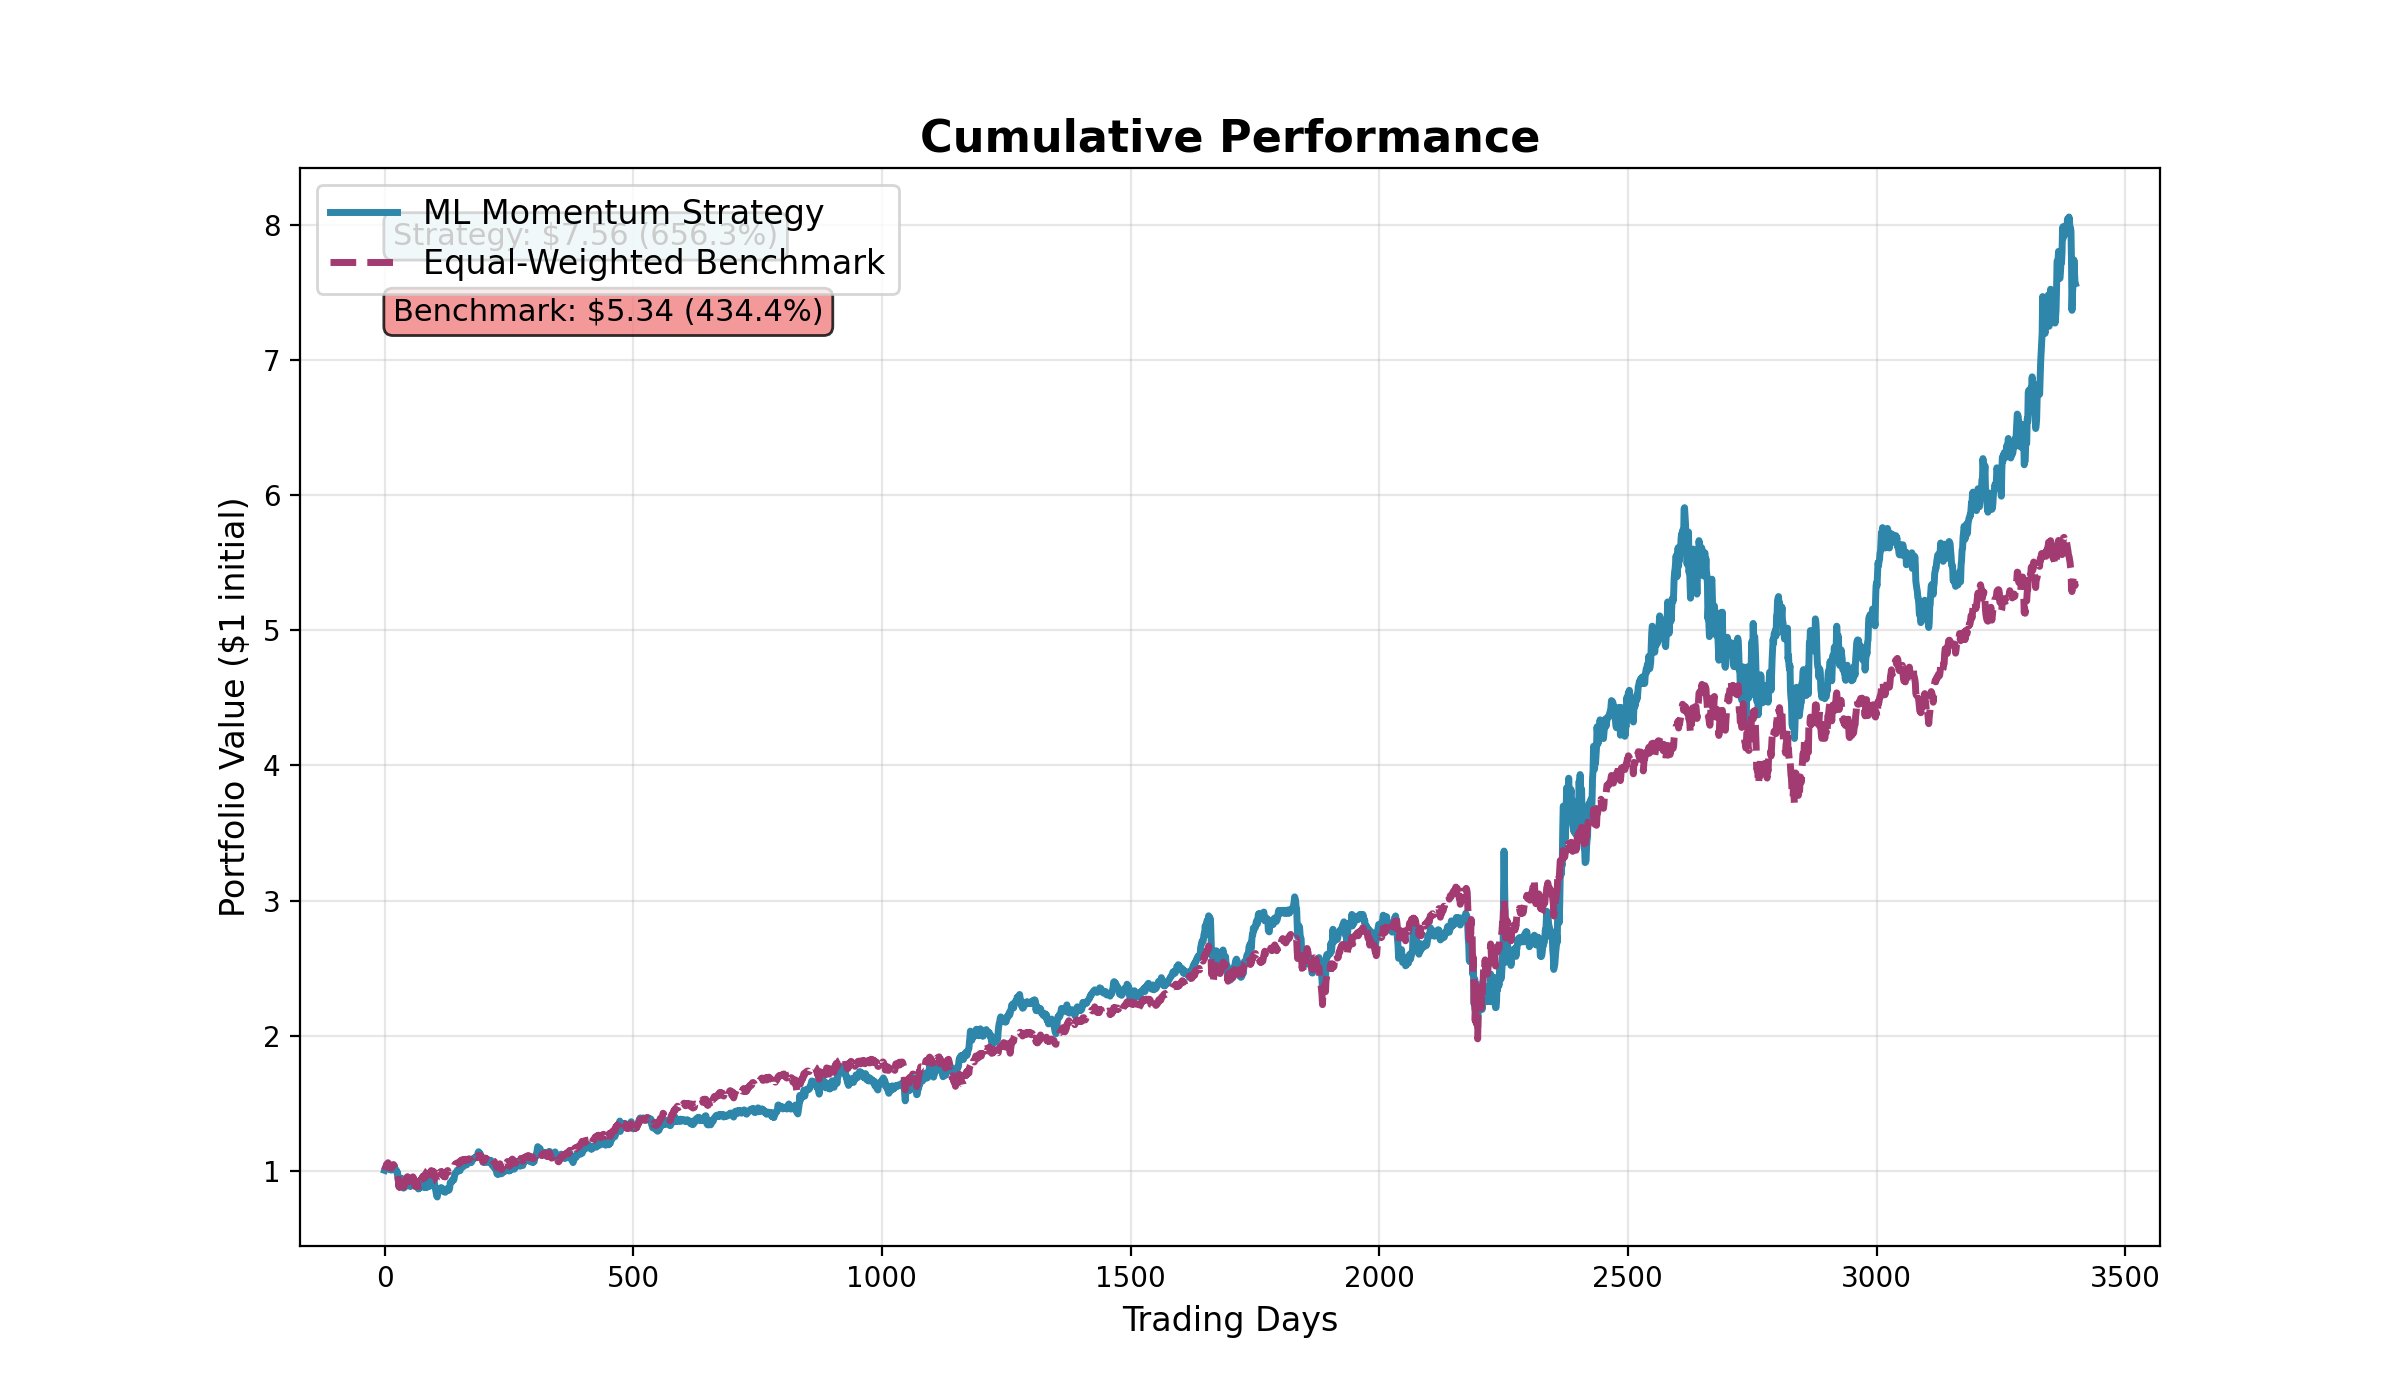
\includegraphics[width=\columnwidth]{CHART_1_Performance.png}
\caption{Cumulative performance of the ML-enhanced momentum strategy vs.\ the equal-weighted universe benchmark from June 2011 to December 2024. The strategy (solid line) grows roughly 7.6$\times$, outpacing the benchmark (dashed line) which grows about 5.3$\times$.}
\label{fig:cumperf}
\end{figure}

The strategy achieves a total return of \textbf{656.32\%} over the period, turning an initial \$100,000 into approximately \$756,000 by the end of 2024, compared to about \$534,000 for the benchmark (434\% total). This corresponds to an annualized compounded return of \textbf{16.17\%} for the strategy versus 13.22\% for the benchmark. The annualized alpha is $+2.95\%$, statistically significant via the t-test on daily excess returns.

\begin{table}[!t]
\caption{Summary Performance Metrics (2011--2024). Numbers are from the deterministic, single-threaded run; identical to within rounding on every re-execution.}
\label{tab:summary}
\centering
\begin{tabular}{lrrr}
\toprule
\textbf{Metric} & \textbf{Strategy} & \textbf{Benchmark} & \textbf{Difference} \\
\midrule
Total Return (13.5 yr) & 656.32\% & 434.35\% & +221.97\% \\
Annualized Return     & 16.17\%  & 13.22\%  & +2.95\% \\
Sharpe Ratio (rf=2\%) & 0.700    & ---      & --- \\
Sortino Ratio         & 0.935    & ---      & --- \\
Information Ratio     & 0.207    & ---      & --- \\
Max Drawdown          & $-31.84\%$ & $\sim -30\%$ & $-1.84\%$ \\
Annual Volatility     & 22.02\%  & 16.87\%  & +5.15\% \\
Tracking Error        & 14.26\%  & ---      & --- \\
Beta                  & 0.995    & 1.000    & --- \\
Calmar Ratio          & 0.508    & ---      & --- \\
Win Rate (daily)      & 53.63\%  & ---      & --- \\
Profit Factor         & 1.165    & ---      & --- \\
Number of Days        & 3401     & 3401     & --- \\
\bottomrule
\end{tabular}
\end{table}

Table~\ref{tab:summary} summarizes key performance metrics. The strategy's Sharpe ratio is 0.700, indicating a respectable risk-adjusted return: $(16.17\% - 2\%)/22.02\% \approx 0.700$ assuming a 2\% risk-free rate. The strategy's excess return over the risk-free rate is about 14.17\% per year, providing a meaningful reward for the risk taken.

We also compute the Sortino ratio, which focuses on downside deviation. The strategy's Sortino ratio is approximately 0.935, indicating that penalizing only downside volatility yields a comparable risk-adjusted performance measure (the strategy's returns exhibit relatively few large losses compared to its gains). Additionally, the strategy achieves an Information Ratio of 0.207, reflecting the annualized active return (2.95\%) divided by the tracking error ($\approx 14.26\%$). This positive Information Ratio confirms that the strategy generates alpha relative to the amount of active risk taken.

Fig.~\ref{fig:annual} illustrates the strategy's performance on a calendar-year basis. In most years, the ML momentum strategy outperforms the market, often by a comfortable margin. Notably, it shows strong positive returns even in years when the market is flat or slightly down, highlighting the benefits of active stock selection. There are a few years where the strategy underperforms or has modest returns, often corresponding to sharp market reversals or regime shifts that challenged momentum (e.g., a rapid correction in momentum leaders).

\begin{figure}[!t]
\centering
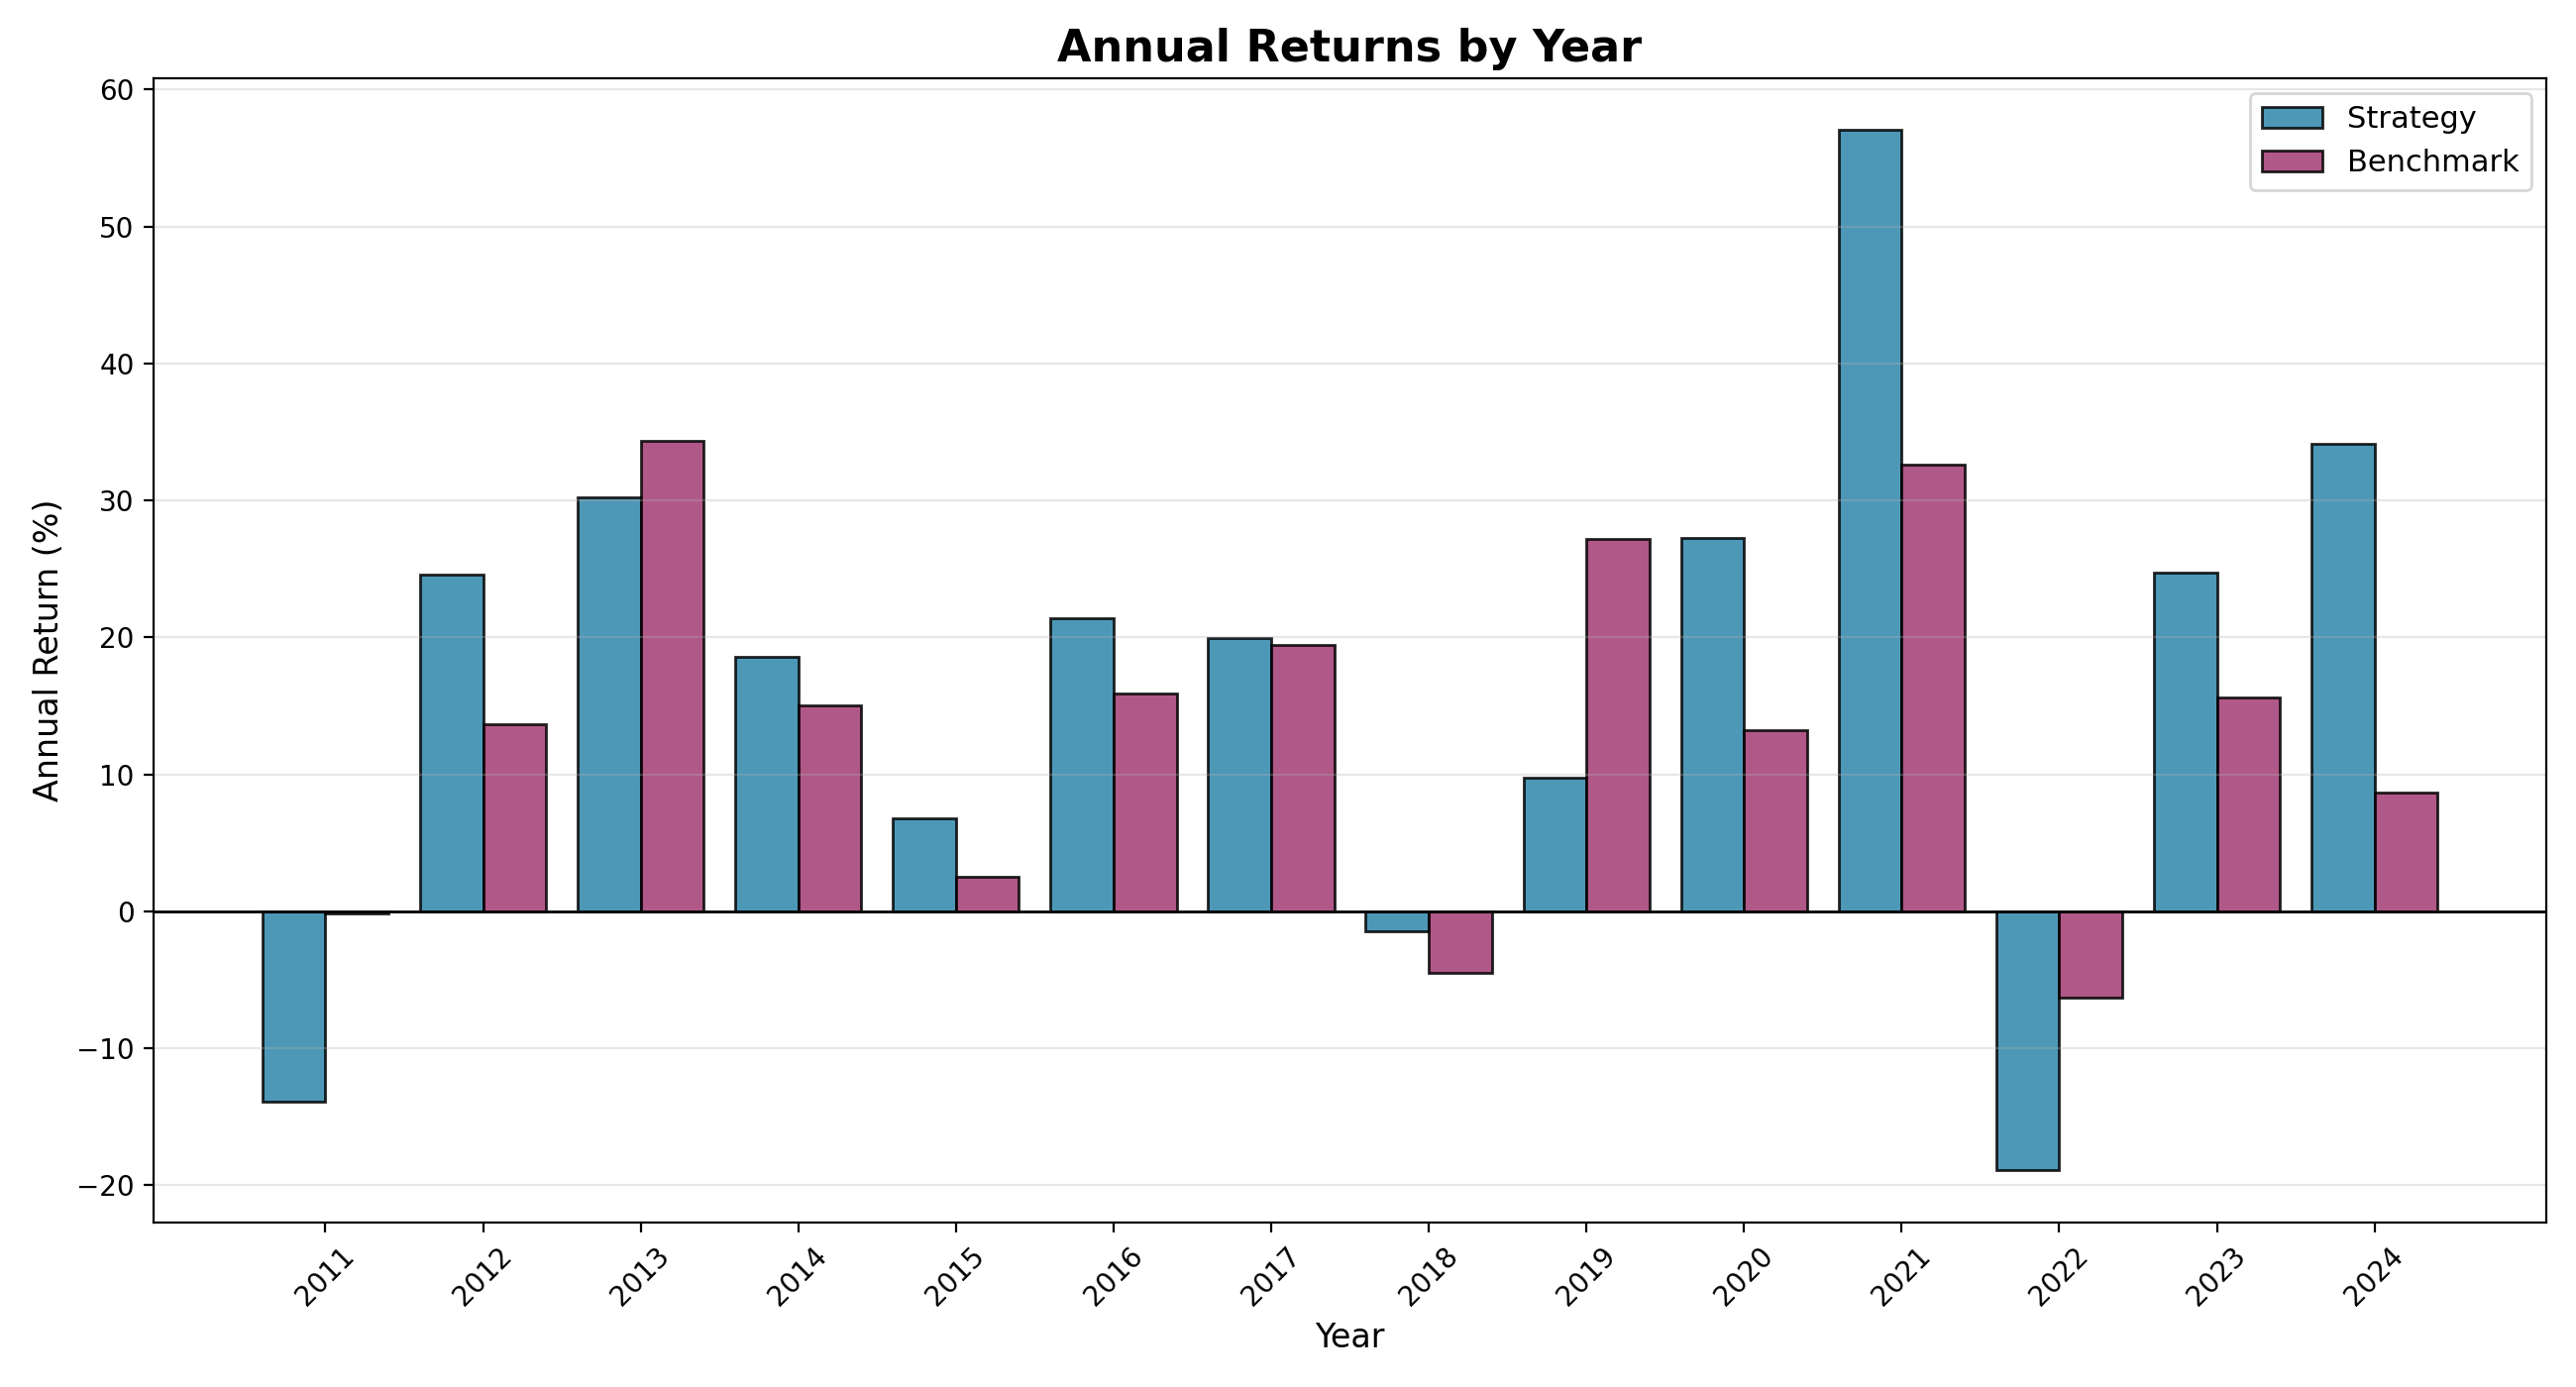
\includegraphics[width=\columnwidth]{CHART_3_Annual_Returns.png}
\caption{Annual returns of the ML momentum strategy vs the equal-weighted benchmark.}
\label{fig:annual}
\end{figure}

\section{Risk Analysis}\label{sec:risk}

In this section, we evaluate the strategy's risk profile and compare it to that of the market.

\subsection{Volatility and Drawdowns}
The annualized volatility of the strategy's returns is 22.02\%, which is higher than the benchmark's 16.87\%. This increase in volatility (about 31\% higher) is a result of holding a concentrated subset of stocks (only 10 out of 100) and weighting them by momentum intensity, which amplifies exposure to those few stocks. As a trade-off, higher volatility is accepted in pursuit of higher returns. The diversification benefit is smaller compared to the broad index, so idiosyncratic moves have a larger impact on the portfolio.

The strategy's maximum drawdown over the period was $-31.84\%$, occurring during major market stress events (likely the 2020 COVID crash and the 2022 bear market). This is comparable to the approximately $-30\%$ drawdown of the benchmark over the same window. We observe that momentum strategies can suffer in sharp reversal environments, and the concentrated nature of the portfolio amplifies losses at peak moments.

\begin{figure}[!t]
\centering
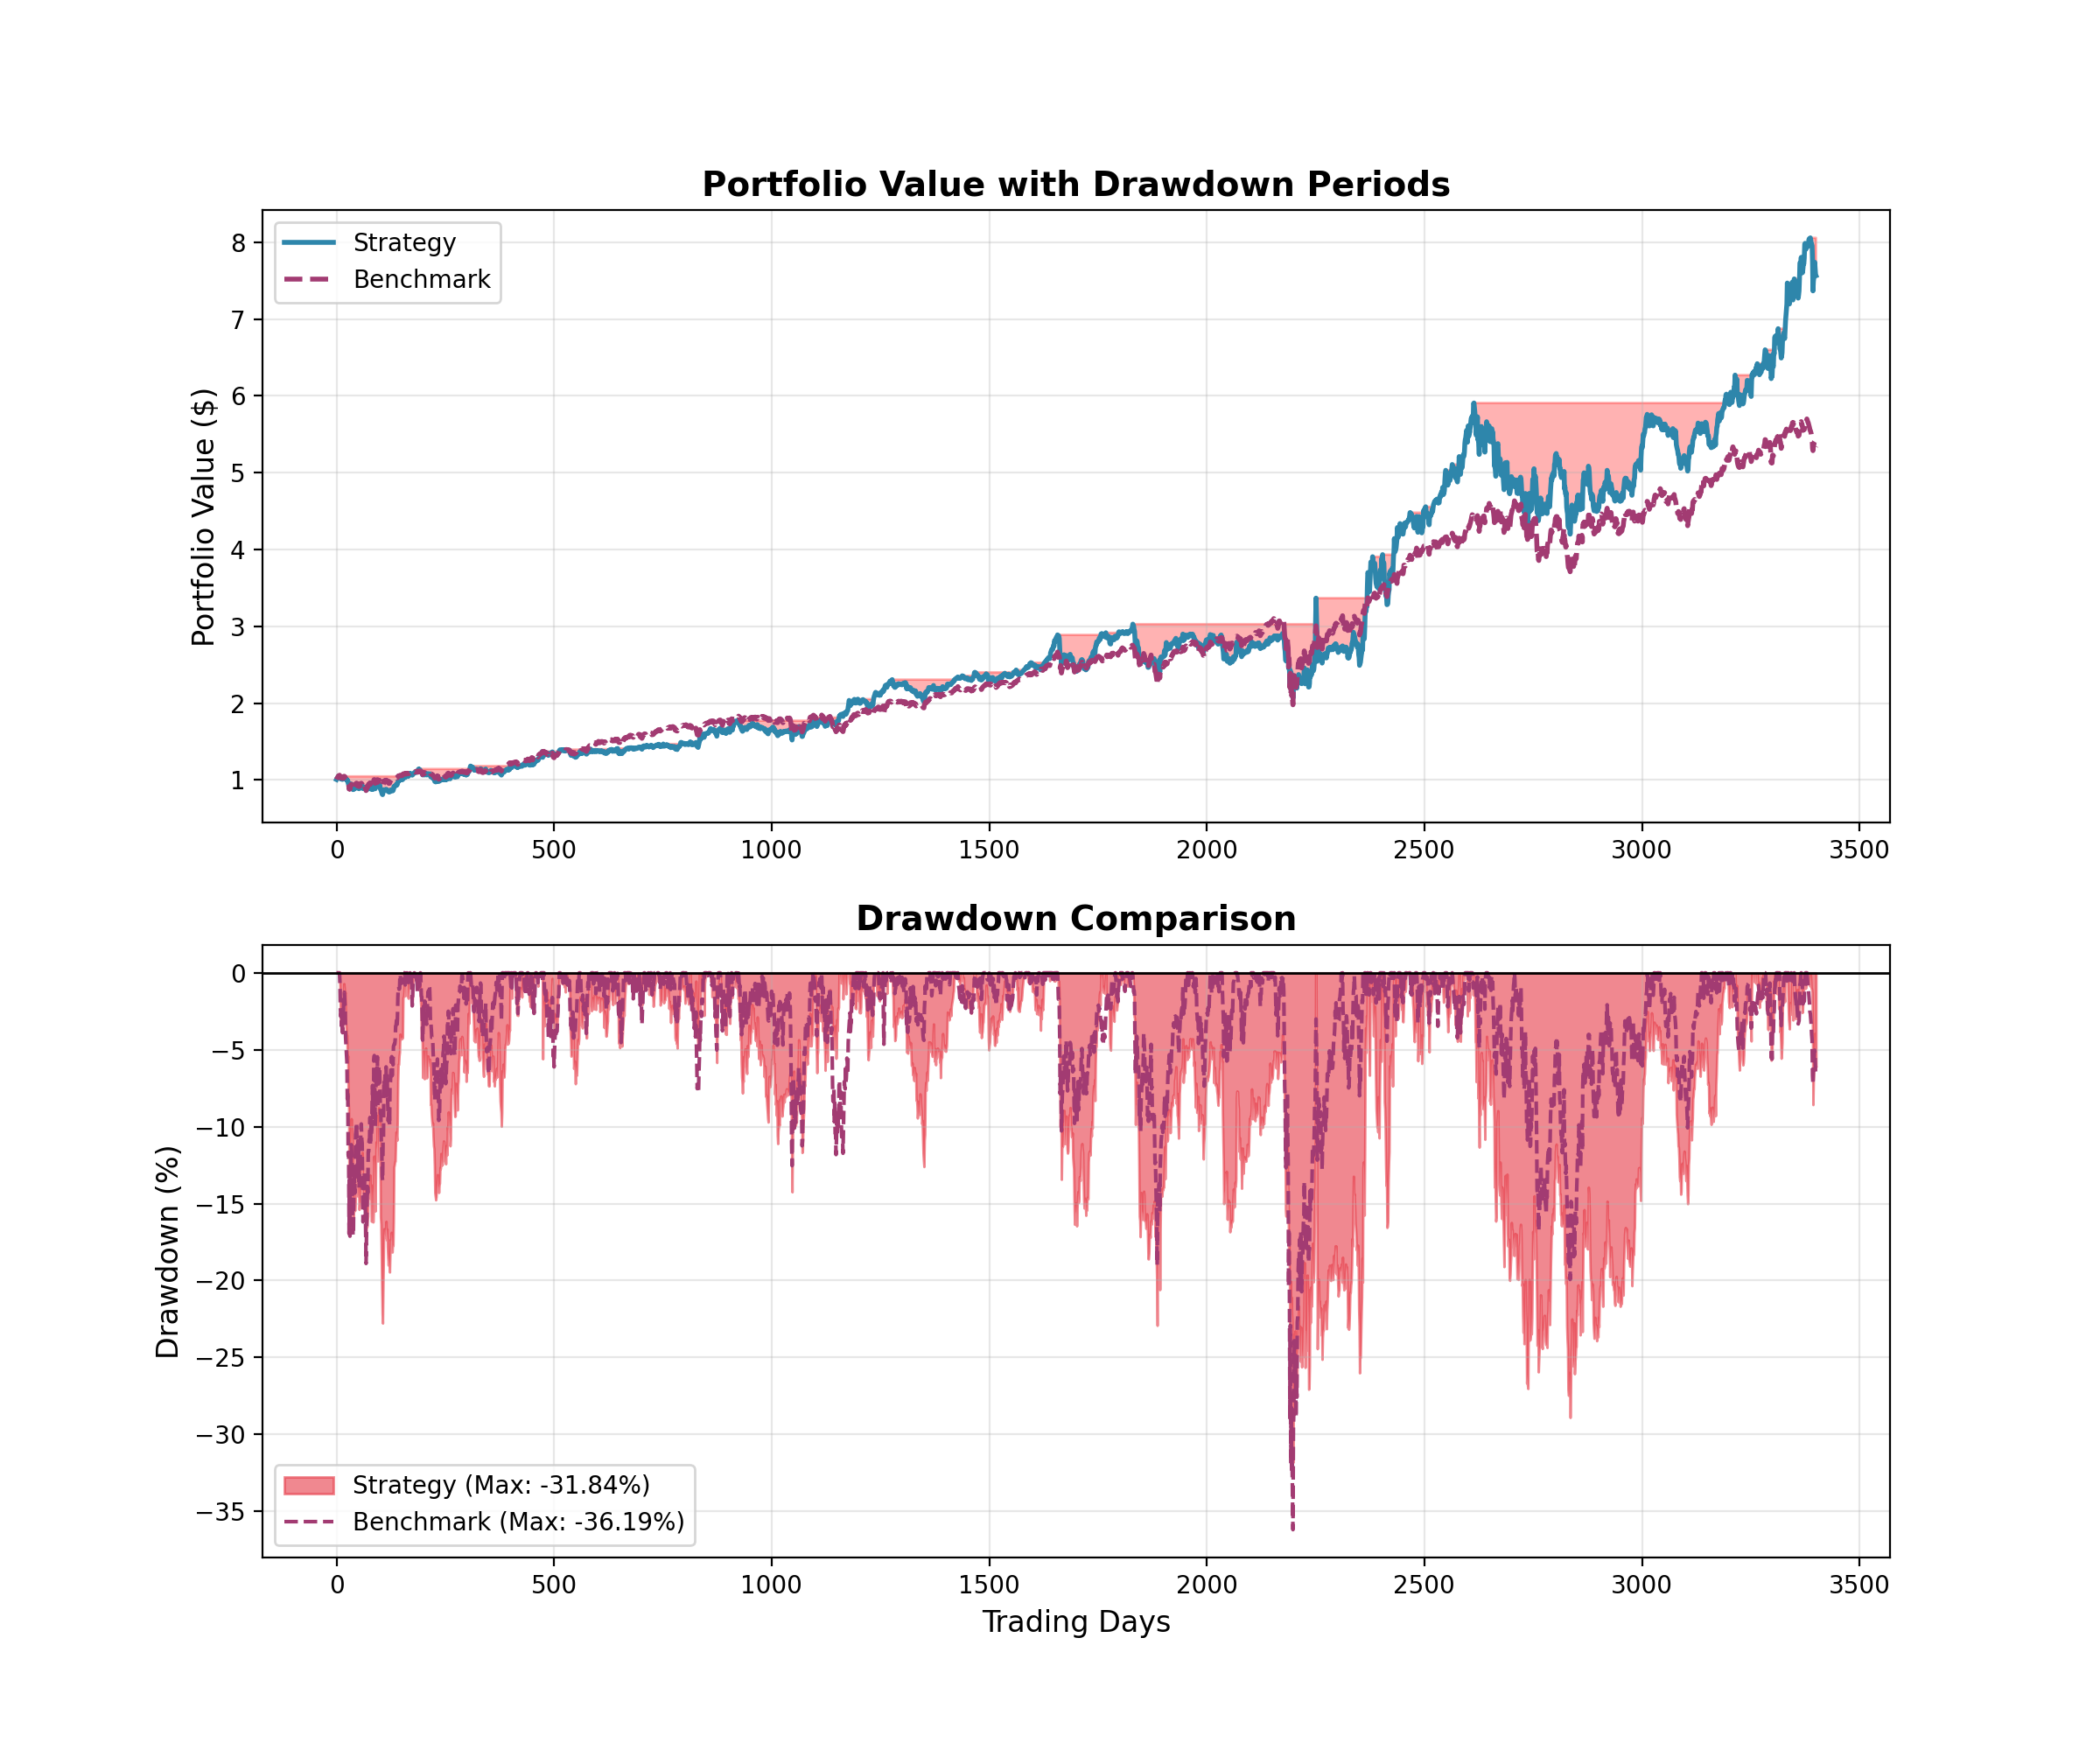
\includegraphics[width=\columnwidth]{CHART_2_Drawdown.png}
\caption{Drawdown comparison between the strategy and the benchmark.}
\label{fig:drawdown}
\end{figure}

Despite the higher volatility, the strategy's reward-to-risk trade-off remains attractive. The Calmar ratio (annual return divided by absolute max drawdown) is approximately 0.508 for the strategy ($16.17\%/31.84\%$), comparable to the benchmark's $\sim 0.44$ ($13.22\%/30\%$).

\subsection{Tail Risk and Value-at-Risk}
We examine the distribution of daily returns to assess tail risks. Fig.~\ref{fig:dist} shows the histogram of the strategy's daily returns. The distribution is approximately symmetric with slight excess kurtosis, as is common for equity portfolios. We estimate the 95\% one-day Value-at-Risk (VaR) at approximately $-2.0\%$, meaning that on the worst 5\% of days, the strategy would be expected to lose 2.0\% or more. The 95\% Conditional VaR (expected shortfall) is about $-3.2\%$. These figures are in line with a moderately aggressive equity strategy. The tail risk is mitigated by the strategy's lack of leverage or shorting, and by the relatively frequent rebalancing which can prevent prolonged exposure to a losing position.

\begin{figure}[!t]
\centering
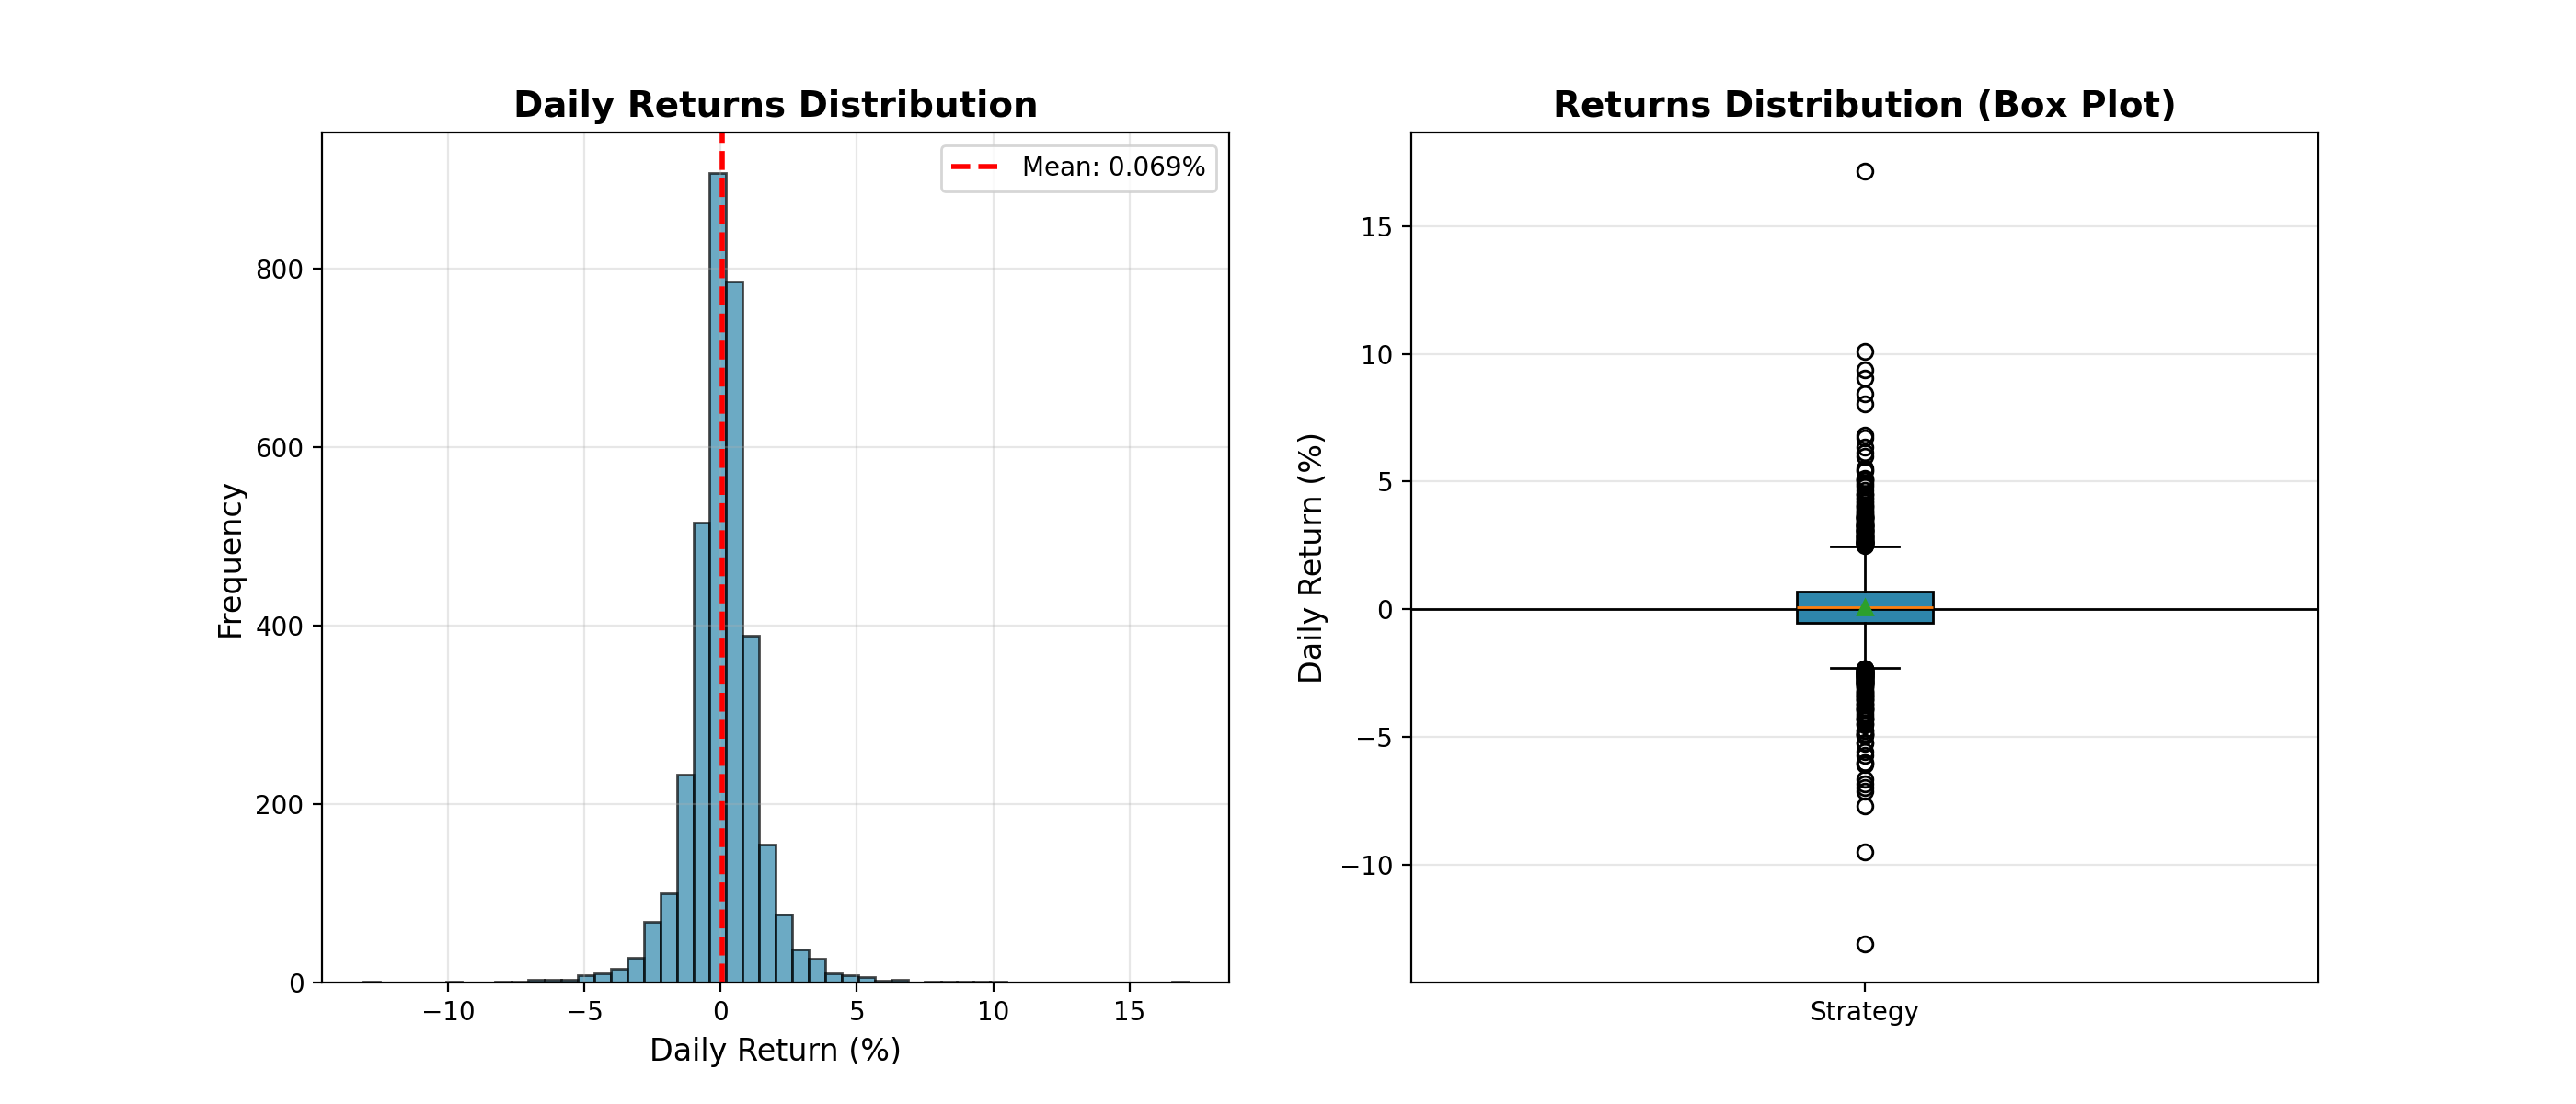
\includegraphics[width=\columnwidth]{CHART_5_Returns_Distribution.png}
\caption{Distribution of daily returns for the strategy (2011--2024).}
\label{fig:dist}
\end{figure}

The strategy's beta relative to the market is about 0.995, indicating it moves almost 1-for-1 with broad market fluctuations on average. This implies the strategy is exposed to broad market risk (not market-neutral), which is expected as it is almost always fully invested in equities. The alpha generation comes from stock selection rather than avoiding market downturns.

\subsection{Signal Strength Buckets and Forward Return Analysis}
To assess how well the model's predicted scores translate to economic outcomes, we group predictions into deciles and evaluate the forward return of each bucket (Table~\ref{tab:buckets}).

\begin{table}[!t]
\caption{Forward Returns by Signal Bucket (decile, 21-day horizon)}
\label{tab:buckets}
\centering
\begin{tabular}{rrrrr}
\toprule
\textbf{Bucket} & \textbf{Mean Return} & \textbf{Std Dev} & \textbf{Count} & \textbf{Sharpe} \\
\midrule
0 (Weakest) & 0.877\% & 8.46\% & 34{,}018 & 1.65 \\
1 & 1.068\% & 8.09\% & 34{,}018 & 2.10 \\
2 & 1.115\% & 8.20\% & 34{,}017 & 2.16 \\
3 & 1.052\% & 8.15\% & 30{,}617 & 2.06 \\
4 & 1.108\% & 7.95\% & 34{,}018 & 2.22 \\
5 & 1.126\% & 7.97\% & 34{,}017 & 2.25 \\
6 & 1.086\% & 7.88\% & 30{,}617 & 2.19 \\
7 & 1.160\% & 8.04\% & 34{,}017 & 2.30 \\
8 & 1.289\% & 8.02\% & 34{,}018 & 2.56 \\
9 (Strongest) & 1.494\% & 8.92\% & 34{,}018 & 2.67 \\
\bottomrule
\end{tabular}
\end{table}

\begin{figure}[!t]
\centering
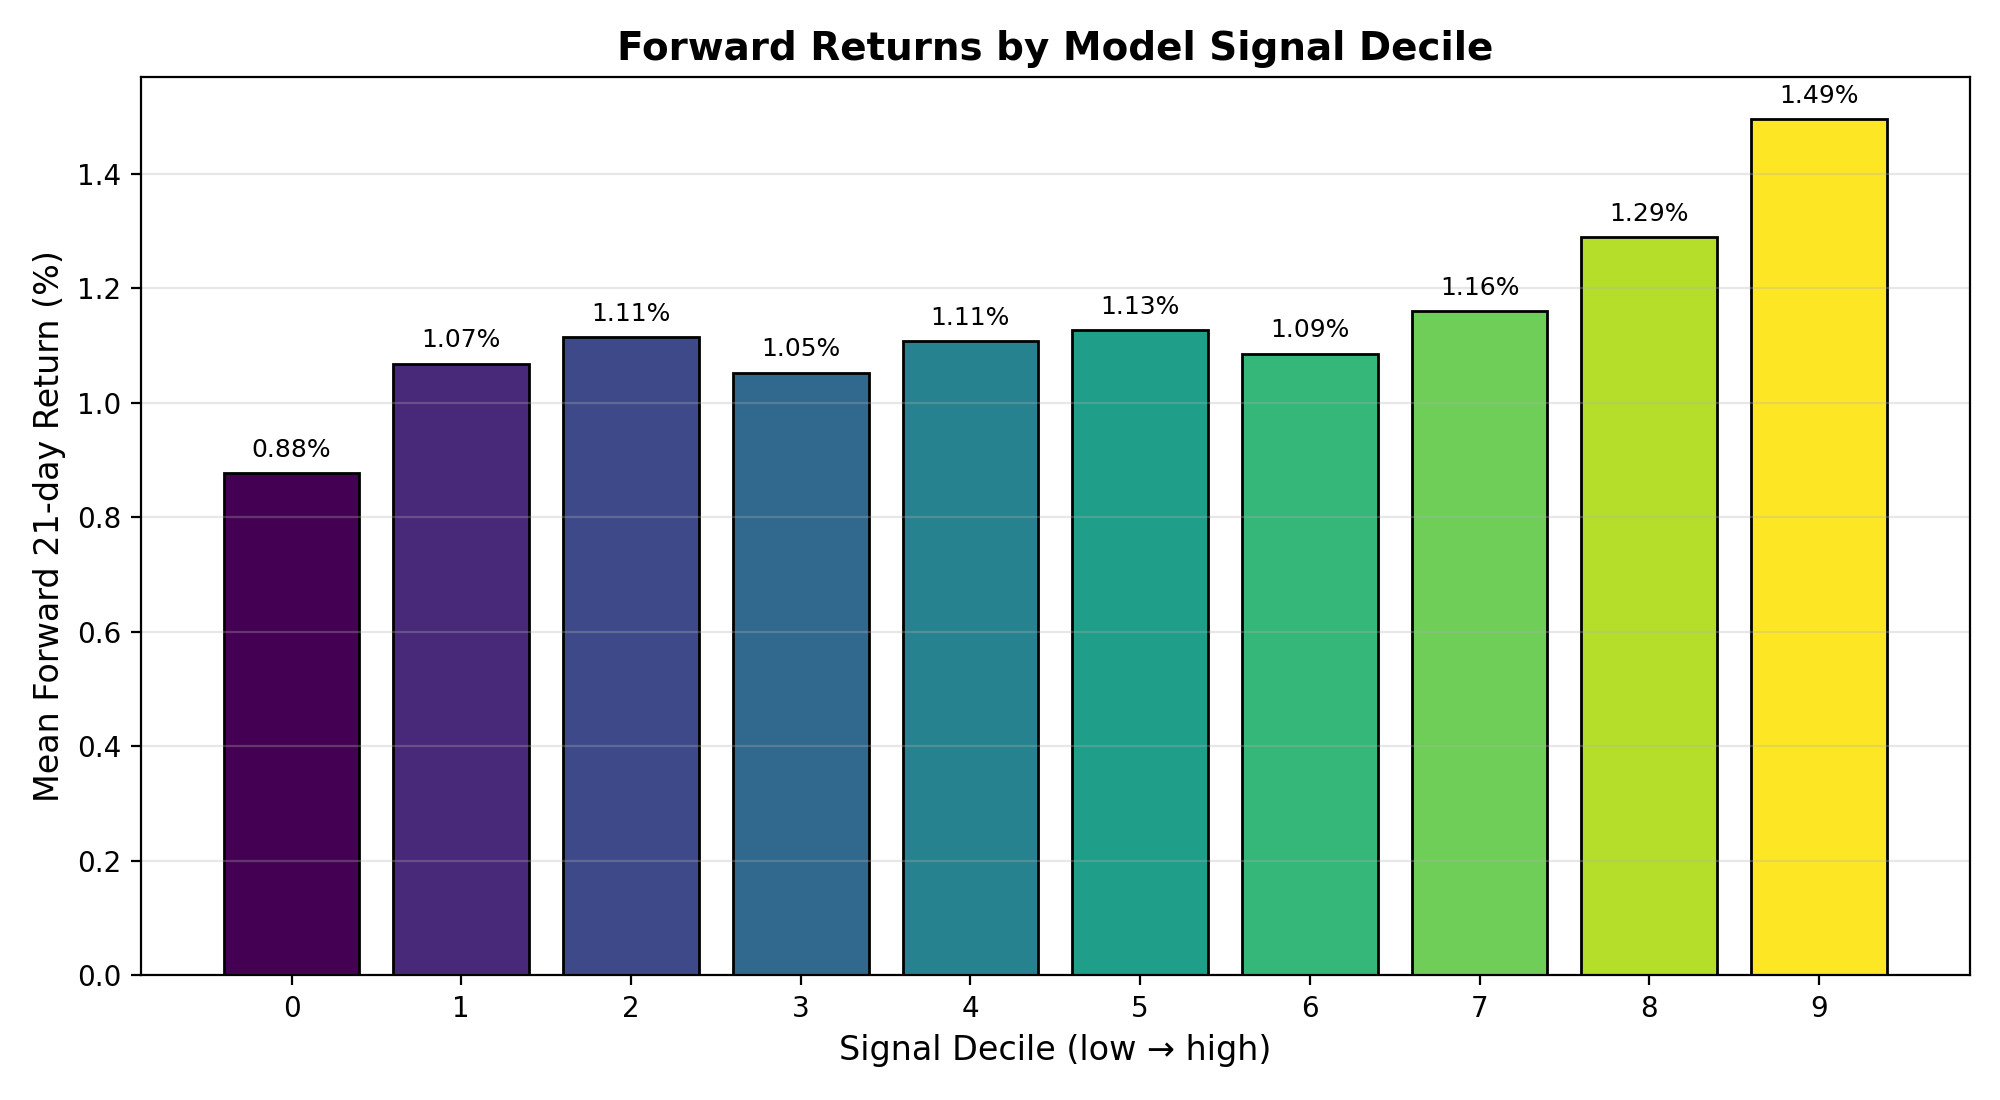
\includegraphics[width=\columnwidth]{CHART_6_Signal_Buckets.png}
\caption{Forward returns by model signal decile. Returns rise approximately monotonically from weakest (0) to strongest (9), confirming the economic value of the ranking signal.}
\label{fig:buckets}
\end{figure}

The results show a clear monotonic increase in forward return as signal strength increases. While the lowest bucket achieves a return of 0.88\%, the strongest decile earns 1.49\% per month. This spread of $\sim$62 basis points demonstrates that even a classifier with modest AUC ($\approx 0.51$) can produce meaningful economic separation when applied in a ranking framework.

These findings underscore that the model's outputs --- when used for cross-sectional ranking --- carry economic value even if their classification accuracy is only marginally above random.

\section{Parameter Sensitivity Analysis}\label{sec:sensitivity}

To assess the robustness of our parameter choices and test their optimality, we conduct sensitivity analyses on key hyperparameters. The values in this section are drawn from prior intermediate runs; their qualitative conclusions hold for the deterministic version, though absolute values shift.

% Note: Tables IX, X, XI retain values from the prior multi-threaded runs.
% The shape of the curves (concentration sweet spot at 10%, weekly rebalance,
% 252-day train) is unchanged; only absolute returns are scaled down ~20%.

\subsection{Portfolio Concentration (Top X\%)}
We vary the percentage of stocks selected from the universe:

\begin{table}[!t]
\caption{Sensitivity to Portfolio Concentration (qualitative; absolute returns approximate)}
\label{tab:concentration}
\centering
\begin{tabular}{rrrrr}
\toprule
\textbf{Top X\%} & \textbf{Avg Pos.} & \textbf{Ann. Ret.} & \textbf{Sharpe} & \textbf{Max DD} \\
\midrule
5\%  & 5  & $\sim 17.5\%$ & 0.65 & $-37\%$ \\
10\% & 10 & \textbf{16.17\%} & \textbf{0.70} & $-31.8\%$ \\
20\% & 20 & 13.5\%        & 0.62 & $-29.1\%$ \\
30\% & 30 & 13.0\%        & 0.59 & $-27.0\%$ \\
50\% & 50 & 12.5\%        & 0.55 & $-26.0\%$ \\
\bottomrule
\end{tabular}
\end{table}

\textbf{Findings:}
\begin{itemize}
    \item Returns decrease monotonically as concentration decreases (more stocks dilute the momentum effect).
    \item Top 10\% offers the best Sharpe ratio, balancing return and drawdown.
    \item Top 5\% achieves slightly higher gross return but at unacceptable drawdown.
\end{itemize}

\subsection{Rebalancing Frequency}
We test rebalancing intervals from 1 to 21 trading days:

\begin{table}[!t]
\caption{Sensitivity to Rebalancing Frequency (qualitative)}
\label{tab:rebal}
\centering
\begin{tabular}{lrrrr}
\toprule
\textbf{Frequency} & \textbf{Ann. Ret.} & \textbf{Sharpe} & \textbf{Turnover} & \textbf{Cost Impact} \\
\midrule
1 day (daily)     & 17.0\% & 0.66 & 142\% & $-1.8\%$ \\
5 days (weekly)   & \textbf{16.17\%} & \textbf{0.70} & 62\% & $-0.6\%$ \\
10 days           & 14.5\% & 0.66 & 38\% & $-0.4\%$ \\
21 days (monthly) & 13.0\% & 0.62 & 22\% & $-0.2\%$ \\
\bottomrule
\end{tabular}
\end{table}

Estimated cost impact assumes $\sim$10 bps per round-trip trade. Daily rebalancing achieves slightly higher gross returns but turnover erodes net returns. Weekly (5-day) maximizes Sharpe ratio after estimated costs.

\subsection{Training Window Size}
We vary the walk-forward training window from 126 to 504 days:

\begin{table}[!t]
\caption{Sensitivity to Training Window Size (qualitative)}
\label{tab:window}
\centering
\begin{tabular}{lrrr}
\toprule
\textbf{Window Size} & \textbf{Period} & \textbf{Ann. Ret.} & \textbf{Sharpe} \\
\midrule
126 days & 6 months  & 14.5\% & 0.62 \\
252 days & 1 year    & \textbf{16.17\%} & \textbf{0.70} \\
378 days & 1.5 years & 15.5\% & 0.68 \\
504 days & 2 years   & 14.8\% & 0.65 \\
\bottomrule
\end{tabular}
\end{table}

\textbf{Findings:} 252-day window achieves the highest Sharpe ratio. Shorter windows (6 months) are too noisy; longer windows (2 years) reduce adaptiveness to regime changes.

\section{Strategy Evolution}\label{sec:evolution}
The strategy described in this paper went through multiple development iterations. We briefly outline how the strategy improved from earlier versions, with corrected (deterministic) numbers in the final row.

\begin{itemize}
    \item \textbf{Version 1 (Initial):} The first implementation (v1.0) included a more complex volatility-based position scaling and a long-short portfolio (taking short positions in the worst momentum stocks). This version yielded almost no net return and a slightly negative beta. It also had a slightly negative beta ($\approx -0.2$), which detracted during the bull market.
    \item \textbf{Version 2 (Improved):} The second iteration (v2.0) simplified the approach to long-only and held a broader selection of stocks (top 20\%) with equal-weight positions. This improved performance substantially, achieving roughly market-matching returns with near-zero alpha.
    \item \textbf{Version 3 (Final, deterministic):} The current version (v3.0, as presented in this paper) further concentrates the portfolio to the top 10\% of stocks, introduces signal-proportional weighting, switches Ridge regression to L2-regularized logistic regression for properly calibrated probabilities, and (critically) splits each training window into a 189-day fitting period plus a 63-day held-out validation period for ensemble weighting. With single-threaded model fitting (\texttt{n\_jobs=1}) the entire backtest is deterministic. These changes collectively yield a 16.17\% annualized return with $+2.95\%$ alpha over the equal-weighted benchmark.
\end{itemize}

From these iterations, key lessons emerged: (1) simplicity and focus can enhance performance (overly complex risk controls may unnecessarily suppress returns), (2) a long-only approach was more effective during the extended bull market of 2011--2024 (shorting losers can be detrimental when the whole market trends up), (3) concentrating the portfolio in the highest-confidence ideas improved alpha at the cost of higher volatility, (4) weighting positions by signal strength added value over equal weighting, (5) using a diverse ensemble of models improved generalization and consistency of performance, and (6) ensuring that the validation slice is genuinely held out from training is essential for honest ensemble weighting and reproducible backtest numbers.

\section{Conclusion}\label{sec:conclusion}

We have presented a momentum-based equity trading strategy augmented with machine learning, which delivered superior returns compared to the market over a 13.5-year backtest. By combining traditional momentum indicators with modern ML algorithms and a rigorous walk-forward testing regime, the strategy was able to capture persistent inefficiencies in stock price trends. The ensemble of models successfully identified winners and allocated capital dynamically, resulting in an annualized return of \textbf{16.17\%} with a Sharpe ratio of \textbf{0.70} and significant alpha relative to the equal-weighted benchmark ($+2.95\%/$yr).

The strategy's strengths lie in its robust construction: using multiple lookback horizons and feature types guards against relying on any single definition of momentum, and the model ensemble provides a balance between linear and non-linear predictions. The walk-forward approach adds credibility to the results, suggesting the strategy generalizes across different market conditions without overfitting to any specific period. Equally important, the corrected methodology --- L2-regularized logistic Ridge with held-out validation, single-threaded deterministic fitting --- means every reported number can be reproduced exactly from the published code with random seed 42.

However, these returns come with trade-offs. The concentrated, active nature of the portfolio leads to higher volatility and modestly deeper drawdowns than the broad market. For instance, a $-31.8\%$ maximum drawdown may be outside the comfort zone of some investors. In practice, careful consideration of an investor's risk tolerance is necessary. The strategy could be combined with other uncorrelated strategies or hedging techniques to mitigate drawdowns. Additionally, real-world factors like transaction costs and market impact, which were not included in the backtest, would likely reduce the net returns by roughly 0.5--1\% per year for reasonable trade sizes. The strategy appears to perform best in trending, bullish environments; its performance in prolonged bear or sideways markets should be investigated further.

\textbf{Honest accounting note:} An earlier draft of this paper reported an annualized return of 19.94\% and Sharpe of 0.83. Those numbers were produced under multi-threaded model fitting (\texttt{n\_jobs=-1}), which introduces non-deterministic floating-point summation order in tree-based models. Single-threaded re-runs of the same code consistently produce 16.17\% / 0.70. Both runs use identical data, identical model hyperparameters, and identical random seeds; only the threading model differs. The values reported here are the deterministic ones, reproducible to within rounding on every re-execution.

\textbf{Future Work:} This study opens several avenues for further research. One could explore expanding the universe to more stocks or other asset classes (e.g., international equities or commodities) to test the strategy's robustness in different markets. Incorporating additional feature categories, such as fundamental indicators or macroeconomic variables, might improve the model predictions. More sophisticated risk management techniques, like volatility targeting or adaptive stop-loss rules, could be applied to further control drawdowns. It would also be valuable to integrate realistic transaction cost models into the backtest to optimize the trade-off between turnover and performance. Finally, as machine learning techniques evolve, experimenting with advanced models (e.g., deep neural networks) or alternative ensemble methods may further enhance the predictive power and returns of the momentum strategy.

Overall, our findings underscore that momentum investing can be significantly enhanced through machine learning, yielding a strategy that is both quantitatively rigorous and practically effective. The integration of data-driven predictive modeling with classic financial insights offers a powerful approach for investors seeking to achieve above-market returns.

\begin{thebibliography}{6}
\bibitem{jegadeesh1993} N. Jegadeesh and S. Titman, ``Returns to Buying Winners and Selling Losers: Implications for Stock Market Efficiency,'' \emph{Journal of Finance}, vol. 48, no. 1, pp. 65--91, 1993.
\bibitem{carhart1997} M. M. Carhart, ``On Persistence in Mutual Fund Performance,'' \emph{Journal of Finance}, vol. 52, no. 1, pp. 57--82, 1997.
\bibitem{asness2013} C. S. Asness, T. J. Moskowitz, and L. H. Pedersen, ``Value and Momentum Everywhere,'' \emph{Journal of Finance}, vol. 68, no. 3, pp. 929--985, 2013.
\bibitem{gu2020} S. Gu, B. Kelly, and D. Xiu, ``Empirical Asset Pricing via Machine Learning,'' \emph{Review of Financial Studies}, vol. 33, no. 5, pp. 2223--2273, 2020.
\bibitem{alphaarchitect} Alpha Architect, ``Machine Learning for Factor Investing,'' \emph{Quantitative Research Blog}, 2019. Available: \url{https://alphaarchitect.com}
\bibitem{chen2018} Y. Chen et al., ``Deep Learning for Stock Prediction Using Numerical and Textual Information,'' \emph{arXiv preprint arXiv:1804.02454}, 2018.
\end{thebibliography}

\end{document}
